\chapter{Results and discussion}

You should have a separate chapter for presenting your results (generated by the stuff described previously, in our case in \cref{chap:math}). Remember that your work needs to be validated rigorously, and no one will believe you if you just say that `it worked well for you'.

Instead, try some of the following:
\begin{itemize}
\item State a hypothesis and prove it statistically
\item Show plots with measurements that you did to prove your results (e.g. speedup). Use either \texttt{R} and \texttt{ggplot}, or Python with \texttt{matplotlib} to generate the plots.\footnote{Honestly, the plots from \texttt{ggplot} look \underline{much} better.} Save them as PDF to avoid printing pixels (as in \cref{fig:f}).
\item Compare with other similar software/theses/authors/results, if possible
\item Show example source code (e.g. for demonstrating how easily your results can be used)
\item Include a `toy problem' for demonstrating the basic functionality of your approach and detail all important properties and results on that
\item Include clear pictures of `inputs' and `outputs' of all your algorithms, if applicable
\end{itemize}

\begin{figure}
\centering
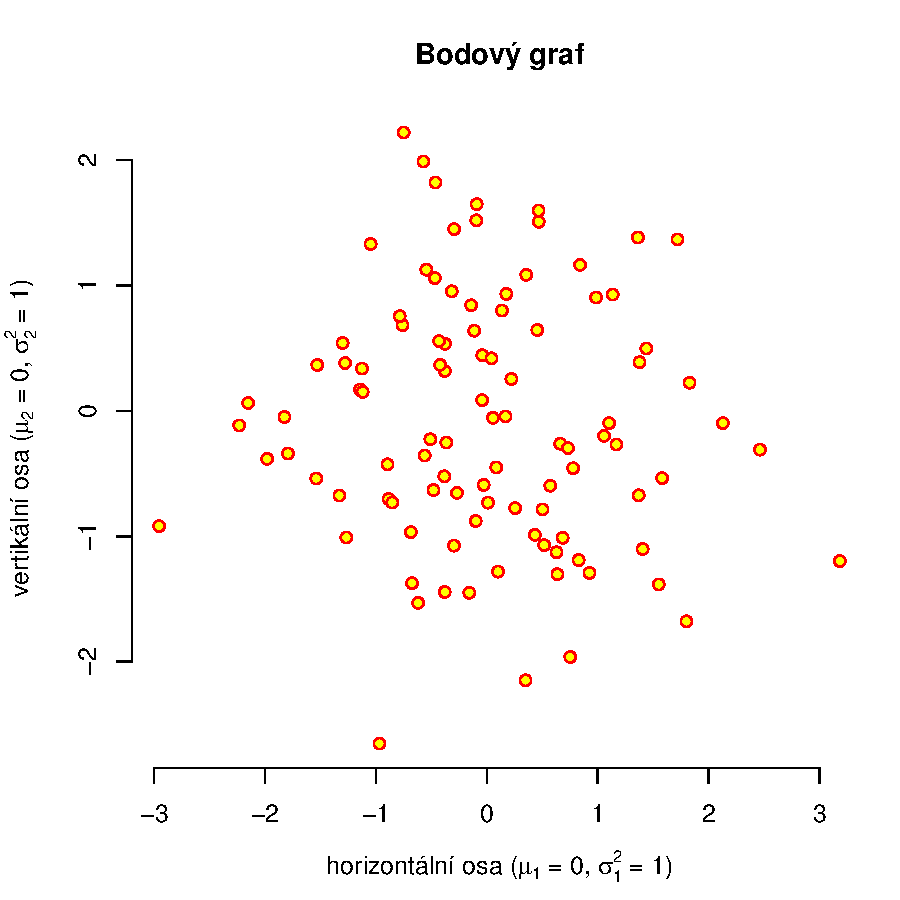
\includegraphics[width=.6\linewidth]{img/ukazka-obr01.pdf}
\caption{This caption is a friendly reminder to never insert figures ``in text,'' without a floating environment, unless explicitly needed for maintaining the text flow (e.g., the figure is small and developing with the text, like some of the centered equations, as in \cref{thm:y}). All figures \emph{must} be referenced by number from the text (so that the reader can find them when he reads the text) and properly captioned (so that the reader can interpret the figure even if he looks at it before reading the text --- reviewers love to do that).}
\label{fig:f}
\end{figure}

It is sometimes convenient (even recommended by some journals, including Cell) to name the results sub-sections so that they state what exactly has been achieved. Examples follow.

\section{SuperProgram is faster than OldAlgorithm}
\subsection{Scalability estimation}
\subsection{Precision of the results}
\section{Weird theorem is proven by induction}
\section{Amount of code reduced by CodeRedTool}
\subsection{Example}
\subsection{Performance on real codebases}
\section{\sloppy NeuroticHelper improves neural network learning}

\section{What is a discussion?}
After you present the results and show that your contribution works, it is important to \emph{interpret} them, showing what they mean for the more general public.

Separate discussion sections are common in life sciences where ambiguity is common and intuition is sometimes the only thing that the authors have; exact sciences and mathematicians do not use them as often. Despite of that, it is nice to precisely set your output into the existing environment, answering:
\begin{itemize}
\item What is the potential application of the result?
\item Does the result solve a problem that other people encountered?
\item Did the results point to any new (surprising) facts?
\item Why is the result important for your future work (or work of anyone other)?
\item Can the results be used to replace (and improve) anything that is used currently?
\end{itemize}

If you do not know the answers, you may want to ask the supervisor. Also, do not worry if the discussion section is half-empty or completely pointless; you may remove it completely without much consequence. It is just a bachelor thesis, not a world-saving avenger thesis.
